\documentclass{article}
\usepackage[left=2cm,right=2cm,top=3cm,bottom=3cm,letterpaper]{geometry}
\usepackage[spanish]{babel}
\usepackage[utf8]{inputenc}
\usepackage{amsmath}
\usepackage{graphicx}

\title{C4.5}
\author{Adolfo Marín Arriaga \and Juan Carlos López López \and Luis Rodrigo Rojo Morales}
\date{\today\\}

\begin{document}
 \maketitle
 
 \begin{itemize}
 \item Evaluación de patrones\\\\
 El atributo que asegura que una persona esté en la clase $>$50k es el capital gain, siempre y cuando sea mayor a 6849. En el caso en que sea menor o igual a esa cantidad se toman en consideración otros atributos, principalmente el estado civil, pues si una persona tiene como estado civil Divorced, Married-spouse-absent, Separated o Widowed caeran en la clase $<=$50k. En el caso en que tenga estado civil Married-AF-spouse, se depende únicamente del atributo educación para saber en qué clase cae la persona, y analizando el árbol generado, las personas que tienen educación Bachelors, Some-college o Assoc-voc caeran en la clase $>50k$, y los restantes tipos de educación caeran en $<=$50k. En el caso en que la persona tenga estado civil Married-civ-spouse, se tienen que verificar diversos atributos para al final obtener la predicción de su clase, esto si su educación es distinta a 9th, pues en este caso caera en la clase $<=$50k.
 
  \item Clasificadores para la comparación\\\\
  Para la comparación, los árboles C4.5, es decir, los clasificadores  que se usaron son los del archivo AlgoritmoC45.java que es nuestra implementación y el de la biblioteca J48 en Weka, pues de igual forma se planeaba usar alguna biblioteca de R pero la única que encontramos es C50, y ésta solo contiene una mejora de C4.5 (C5.0).
  \item Primer clasificador\\\\
  Usando el de AlgoritmoC45.java para clasificar los elementos que vienen en el archivo AdultPrepoc.csv nos da el siguiente resultado tentativo:\\
  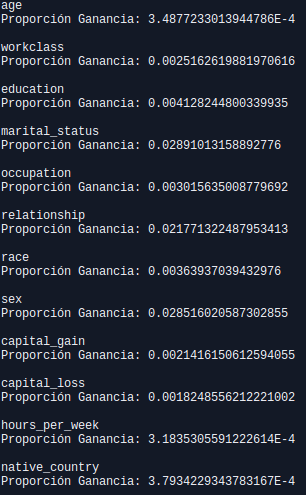
\includegraphics[scale=0.6]{c45java}
  \item Segundo clasificador\\\\
  Usando la biblioteca J48 de Weka para clasificar los elementos que vienen en el archivo AdultDataSetTest.csv nos da el resultado:\\
  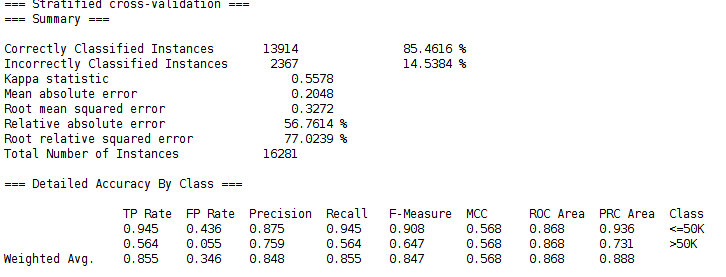
\includegraphics[scale=.9]{c45weka}\\
  \item Comparación\\
  El primer clasificador aún está en la fase de pruebas.\\
  El segundo clasificador clasificó bien a 13914 personas y mal a 2367 personas (14.04\%).\\
  El primer clasificador acertó en el ? de los casos.\\
  El segundo clasificador acertó en el 85.46\% de los casos.\\
 \end{itemize}
 
\end{document}
